\chapter{Estado de la Cuestión}
\label{cap:estadoDeLaCuestion}

En este capítulo, se estudiarán detalladamente las simulaciones basadas en agentes de inteligencia artificial y modelos de lenguaje, así como las complejidades en las relaciones sociales y la interacción persona-ordenador. El objetivo fundamental es contextualizar la evolución histórica y actual de estos temas, destacando la relevancia de su estudio y desarrollo, subrayando la importancia de que estos sistemas puedan ser fácilmente extensibles y utilizados por profesionales de distintos ámbitos. El capítulo se dividirá en varios puntos, los cuales se pueden englobar en dos secciones.

La primera sección del estado de la cuestión se centra en las simulaciones basadas en agentes y su aplicación en entornos de inteligencia artificial. Se explorarán los avances tecnológicos, las metodologías y los desarrollos más recientes que han influido en la creación de sistemas de simulación avanzados. Asimismo, se examinará la relación de estos agentes con modelos de lenguaje, identificando los desafíos de esta convergencia tecnológica.

Después, se revisarán los desarrollos más destacados en procesamiento del lenguaje natural (PLN) y cómo estos contribuyen a la mejora de la interacción entre humanos y sistemas de inteligencia artificial. Además, se explorarán los aspectos psicológicos relacionados con las relaciones sociales en el contexto de la informática. También se centrará en la interacción persona-ordenador, se analizarán las tendencias actuales en diseño centrado en el usuario y las estrategias para garantizar que las simulaciones de inteligencia artificial sean accesibles a todos los públicos, independientemente de su desconocimiento sobre la tecnología.

\section{Simulaciones basadas en agentes}
\section{Modelos de lenguaje}
\subsection{Generativos}
\subsection{LLM}
\section{Agentes}

\section{Procesamiento del lenguaje natural}

El procesamiento del lenguaje natural (NLP, por sus siglas en inglés) es una rama de la inteligencia artificial que se enfoca en la interacción entre las computadoras y el lenguaje humano. El objetivo del NLP es permitir que las máquinas comprendan y procesen el lenguaje humano de la misma manera que lo hacen los seres humanos. Esto lo consiguen combinando la lingüística computacional con modelos estadísticos de machine learning y deep learning, pudiendo así interpretar tanto datos de texto como de voz, e incluso imágenes u otros tipos.

A día de hoy, estos sistemas han sido perfeccionados y se utilizan de manera habitual en varios ámbitos como pueden ser la recuperación y extracción de información, la minería de datos, la traducción automática, el análisis de sentimientos o la generación de resúmenes automáticos \citep{hernandez2013aplicaciones}. En el caso del presente estudio, es especialmente interesante la generación de resúmenes automáticos, ya que es una de las extensiones propuestas en los objetivos de realización del trabajo.

En los últimos años, se han propuesto diversos generadores de secuencias. En particular, los que más éxito han tenido son los basados en arquitecturas de aprendizaje profundo (deep learning) \citep{mishra2020deep}. Las definiciones de la figura \ref{fig:resumenTextos} se refieren a los distintos tipos de resúmenes de textos que pueden existir, según \cite{adhikari2020nlp}. 

\begin{figure}[h]
	\centering
	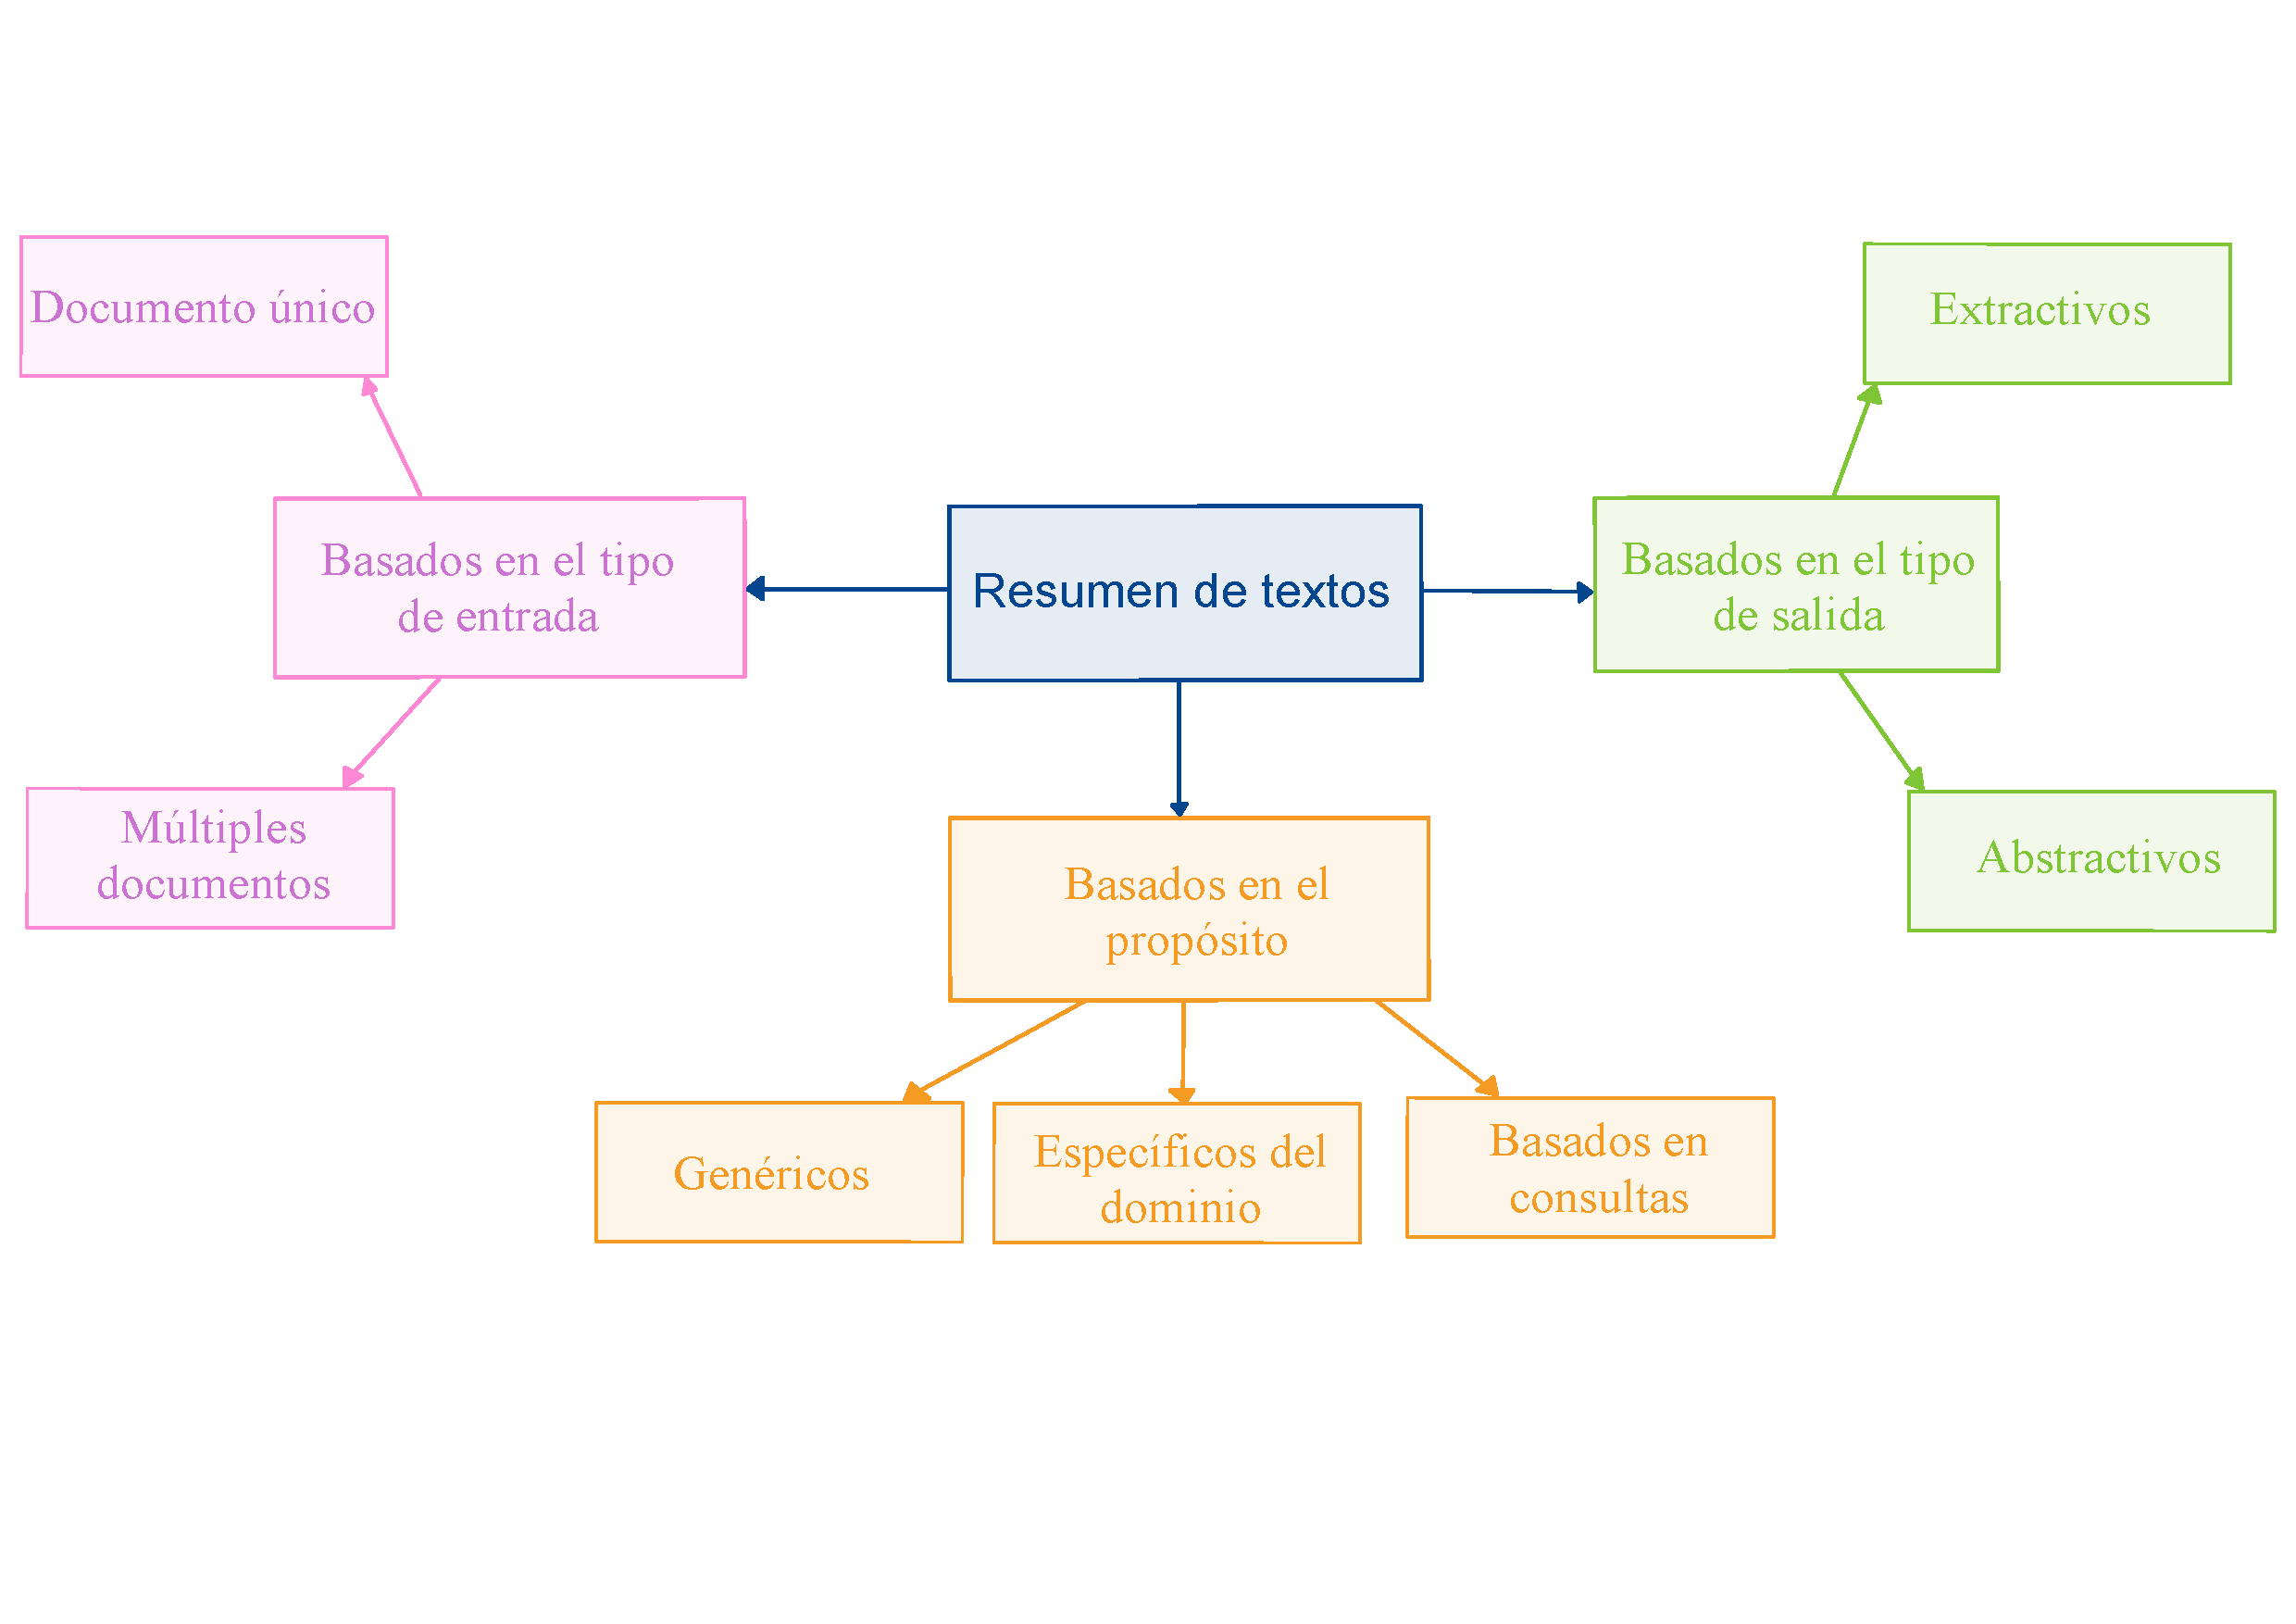
\includegraphics[width = 0.7\textwidth]{Imagenes/Vectorial/resumenTextos.pdf}
	\caption{Resumen de textos (adaptada de \cite{adhikari2020nlp})}
	\label{fig:resumenTextos}
\end{figure}

Los resúmenes extractivos son los que reutilizan las mismas frases existentes en el documento original, los abstractivos son más generales y se centran en los aspectos clave. De manera similar, las técnicas de resumen de un solo documento proporcionan resúmenes del texto de un solo documento, y las de múltiples documentos, generan resúmenes de varios documentos. Además, en la actualidad, hay una necesidad de resumir texto basándose en consultas. Los modelos de resumen basados en consultas proporcionan resúmenes del texto según un área específica descrita por la consulta proporcionada por el usuario, mientras que los resúmenes genéricos son en su mayoría resúmenes abstractos que se centran en el área general del texto de entrada.

\subsection{Interacción persona-ordenador}

\section{Relaciones sociales}
\subsection{Psicología}
\subsection{Informática a lo largo del tiempo}
\section{Extensibilidad y adaptación a todos los públicos}